\chapter[Radiative Transfer Model of the \\Venus Atmosphere]{Radiative Transfer Model of the Venus Atmosphere}

%\section{Introduction}

One key aspect of this research has been to model the microwave and millimeter-wave emission spectra from the surface of Venus and its atmosphere. This is accomplished using a radiative transfer model. The radiative transfer model (RTM) computes the brightness temperature of Venus for a given distribution of atmospheric constituents. The developed RTM is written in a modular way such that any input can be easily changed without changing other aspects. The RTM has the ability to simulate pencil-beam emissions, disk averaged emissions, or the emission over a selected antenna pattern. %This new model provides a more accurate representation of the microwave and millimeter-wave emission spectrum of Venus. 

\section{Theoretical Background}

The emission from the surface of Venus and its atmosphere can be computed using a Radiative Transfer Model (RTM). Radiative transfer is a method to solve for the emission of electromagnetic energy from a medium. In a most basic RTM, it is assumed that the solution for intensity (or brightness temperature) is computed from emissions along an infinitely thin beam (pencil beam). A second assumption is that the atmosphere is in local thermodynamic equilibrium (LTE). LTE implies that for a given moment or snapshot in time the atmosphere is static; that is, the model does not consider atmospheric dynamics when solving the radiative transfer equation. The differential form of the radiative transfer equation is
\begin{equation}\label{eq:rtm-diff}
dI_{\nu}= -\alpha I_{\nu }ds + \alpha J ds
\end{equation}
where $dI_\nu$ is the change in intensity at a given frequency $\nu$ over a path length $ds$, $\alpha$ is the absorption coefficient or attenuation over a path length $ds$, and $J$ is the source function \cite{Liou-2002}. 

In the microwave and millimeter wave regime, effects from scattering approach the Rayleigh limit, and may be neglected without introducing significant error. Therefore the source function $J$ becomes the Plank function.
\begin{equation}\label{eq:rtm-planck}
J_\nu = B_\nu(T) = \frac{h\nu^3}{c^2} \frac{1}{\exp(\frac{h\nu}{kT})-1} \approx \frac{2kT\nu^2}{c^2}
\end{equation}
where $T$ is the temperature in Kelvin, $h$ is Planck's constant, $k$ is Boltzman's constant, and $c$ is the speed of light (Karpowicz \cite{Karpowicz-thesis}). The approximation in equation \ref{eq:rtm-planck} is for cases where $h\nu \ll kT$ (characteristic of centimeter and millimeter-wavelengths) and is known as the Rayleigh-Jeans approximation. %The brightness temperature of the black body can then be directly related to the radiation intensity
%\begin{equation}\label{eq:temp-intensity}
%T_b(\nu) = \frac{\lambda}{2k}I_\nu
%\end{equation}

If equation \ref{eq:rtm-diff} is integrated over the path $s$ it becomes
\begin{equation}\label{eq:rtm-integrated}
I_\nu(s) = I_{\nu,o}(s_0)e^{-\tau_\nu(s_0)}+\int_0^{s_0} \alpha_\nu(s)B_\nu(T) e^{-\tau_\nu(s)}ds 
\end{equation}
where the first term is the intensity at the boundary of the integration and represents contributions to emissions from sources other than those over the path of integration, such as background or surface emission and $\tau$ is the optical depth defined by
\begin{equation}\label{eq:rtm-tau}
\tau_\nu(s) = \int_0^s \alpha_\nu(s') ds'
\end{equation}

For the terrestrial inner planets, the surface term is 
\begin{equation}\label{eq:rtm-surface-term}
\begin{split}
I_{\nu,o}(s_0) =& I_{surf} + I_{cmb}+ I_{down}
\end{split}
\end{equation}
where the first term ($I_{surf}$) is the surface emission, the second term ($I_{cmb}$) is the cosmic microwave background, and the final term ($I_{down}$) is the downwelling radiation from each atmospheric layer. 

While intensity is a quantity often used in solar and ultra-violet remote sensing, it is far more common to use brightness temperature for longer wavelengths such as infrared and microwave. This quantity is found by taking the approximation in Equation \ref{eq:rtm-planck} and solving for $T$. Brightness temperature is defined as,
\begin{equation}\label{eq:rtm-tempbright}
T_b = \frac{Tc^2}{2\nu k}
\end{equation}
Substituting Equations \ref{eq:rtm-planck}, \ref{eq:rtm-tempbright}, and \ref{eq:rtm-surface-term} into \ref{eq:rtm-integrated}, and solving for brightness temperature, the equation for radiative transfer becomes, 
\begin{equation}\label{eq:rtm-tempinte}
\begin{split}
T_b(\nu) = &\left(\epsilon(\theta)T_{surf} + [1-\epsilon(\theta)]e^{-\tau_\nu(s)}T_{cmb}+ T_{down}(\nu)\right)e^{-\tau_\nu(s_0)}\\
&+\int_0^{s_0} \alpha_\nu(s)T(s) e^{-\tau_\nu(s)}ds
\end{split}
\end{equation}
Where $\epsilon(\theta)$ is the surface emissivity, $\theta$ is the transmission angle upward, $T_{surf}$ is the physical surface temperature, $T_{cmb}$ is the cosmic background radiation temperature (2.7K) attenuated while going through the atmosphere (s), $T$ is the physical temperature along the integration path, and finally $T_{down}(\nu)$ is the downwelling radiation from each atmospheric layer attenuated by every layer below it which is expressed as
\begin{equation}
T_{down}(\nu) = \int_{s_0}^{0} \alpha_\nu(s)T(s) e^{-\tau_\nu(s)}
\end{equation}  

The discrete form of \ref{eq:rtm-tempinte} can be expressed as,
\begin{equation}\label{eq:rtm-layers}
\begin{split}
T'_\nu(a) &= \epsilon(\theta)T_{surf} e^{-\tau_{0\rightarrow \infty}} \\
&+ [1-\epsilon(\theta)]T_{cmb}e^{-2\tau_{0\rightarrow\infty}}\\
&+ \sum_{i=1}^N T_i(1-e^{-\tau_i})[1-\epsilon(\theta)] e^{-\tau_{0\rightarrow i-1}} e^{-\tau_{0\rightarrow \infty}}\\
&+ \sum_{i=1}^N T_i(1-e^{-\tau_i}) e^{-\tau_{i+1\rightarrow \infty}} 
\end{split}
\end{equation}
where $a$ is the impact parameter which describes how the ray is emitted from the planet and is computed using a Ray Tracing algorithm and $\tau_{j\rightarrow k}$ is the optical depth from layer j to layer k, 
\begin{equation}\label{eq:rtm-layersum}
\tau_{j\rightarrow k} = \sum_{i=j}^k \tau_i
\end{equation}
$\tau_i$ is the optical depth of layer $i$ and is given by
\begin{equation}\label{eq:rtm-layerdepth}
\tau_i = \int_{s(z=z_i)}^{s(z=z_{i+1})} \alpha(s) ds
\end{equation}
where $z_i$ is the height of the $i^{th}$ layer \cite{Jenkins-2002}. 

To compute the surface emissivity $\epsilon$ the following formula can be used
\begin{equation}\label{eq:rtm-esurf}
\epsilon(\theta) = 1-R_{surf}(\theta)
\end{equation}
where
\begin{equation}\label{eq:rtm-rsurf}
\begin{split}
R_{surf}(\theta) =& \frac{1}{2} \left[ \frac{\cos\theta - \sqrt{\epsilon_d/\eta_1^2-\sin^2\theta}}{\sin\theta + \sqrt{\epsilon_d/\eta_1^2-\sin^2\theta}} \right]^2\\
&+\frac{1}{2} \left[ \frac{\epsilon_d/\eta_1^2 \cos\theta - \sqrt{\epsilon_d/\eta_1^2-\sin^2\theta}}{\epsilon_d/\eta_1^2 \cos\theta + \sqrt{\epsilon_d/\eta_1^2-\sin^2\theta}} \right]^2
\end{split}
\end{equation}
where $\theta$ is the transmission angle upward through the first atmospheric layer and $\eta_1$ is the index of refraction for the first atmospheric layer \cite{Jenkins-2002}. The dielectric constant of the surface $\epsilon_d$ is assumed to have a uniform value of $4.0$ \cite{Pettengill-1992}.

If Equation \ref{eq:rtm-layers} is integrated over all angles of emission and divided by the number of samples taken, the Disk-Averaged brightness can be obtained. This is useful in comparing the model to full-disk observations made of Venus as well as producing residual plots of the planet. The residual plots can be used to find any discrepancies in the Venus atmosphere and allow for identification of atmospheric phenomenon. 

It is also useful to know how each layer of the atmosphere affects the brightness temperature; this can be found through calculation of the weighting function,
\begin{equation}
W_i = (1-e^{\tau_i}) e^{-\tau_{i+1 \rightarrow N}}
\end{equation}

\section{Parameters of the Radiative Transfer Model}
The input parameters of the radiative transfer model (RTM) are the opacity formalisms for the various atmospheric constituents, the index of refraction for each atmospheric layer, the temperature-pressure profiles, and the vertical abundance profiles for the absorbing constituents. Together the last two make up the Thermo-Chemical model of the atmosphere.
\subsection{Temperature-Pressure Profiles}
The temperature-pressure profiles for the atmosphere of Venus have been obtained from the data collected using the Pioneer-Venus sounder and north probes \cite{Seiff-1980}. Figure \ref{fig:temp} shows the temperature as a function of altitude in the Venus atmosphere as reported by the Pioneer-Venus sounder and north probes. Figure \ref{fig:pres} shows the pressures as a function of altitude in the Venus atmosphere as reported by the Pioneer-Venus sounder and north probes.

The sounder probe temperature represents the temperature-pressure profile in the equatorial region of the Venus atmosphere. It is used for latitudes between $-45^\circ$ and $+45^\circ$. The north probe is representative of the polar regions of Venus and it used between $\pm 45^\circ$ and $\pm90^\circ$. A physical surface temperature of 730 K is assumed in this RTM.

\begin{figure}[p]
    \centering
	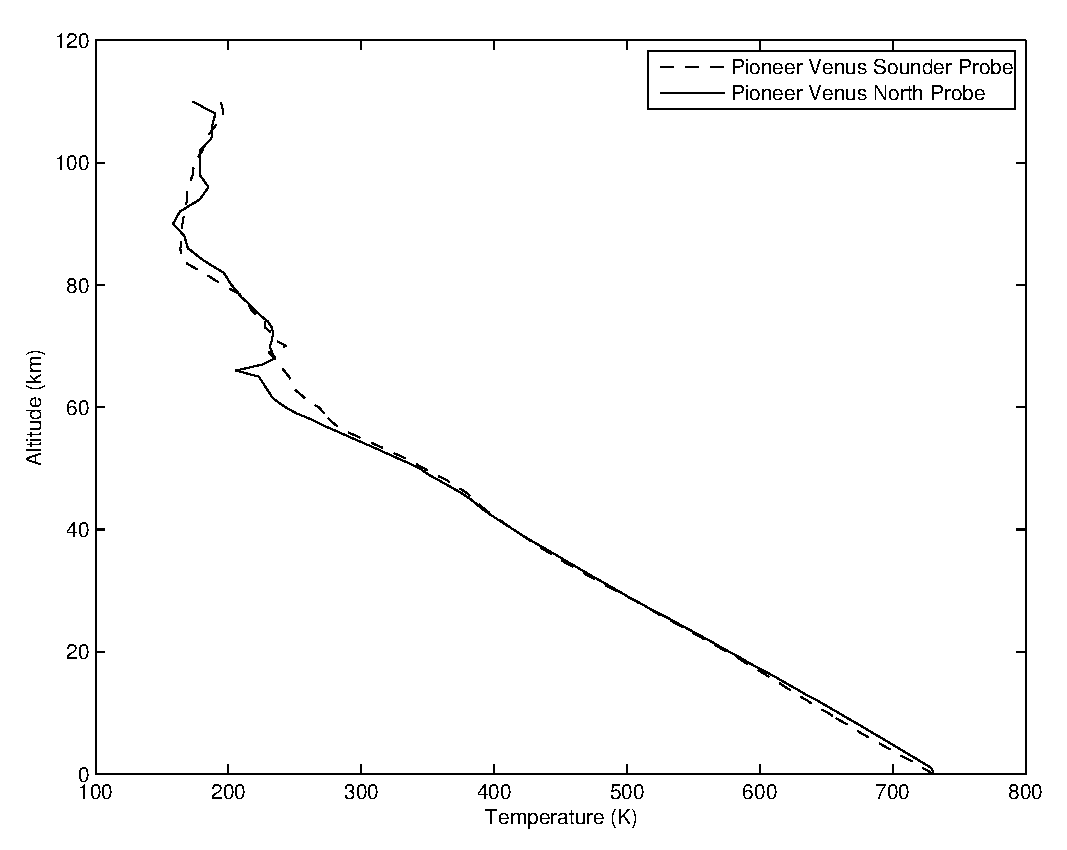
\includegraphics[width=0.7\textwidth]{./rtm/plots/alt-temp.eps}
	\caption{Temperature as a function of altitude in the Venus atmosphere obtained using the Pioneer-Venus sounder and north probes }
		\label{fig:temp}
\end{figure}
\begin{figure}[p]
    \centering
	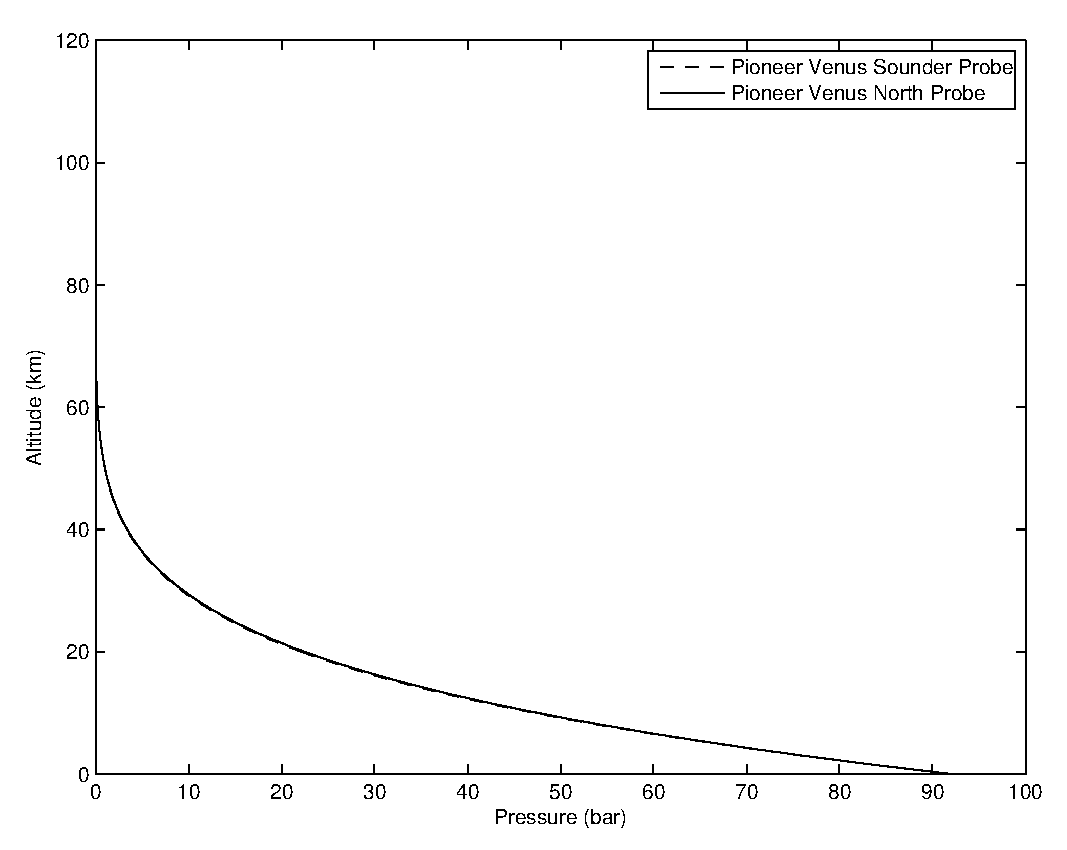
\includegraphics[width=0.7\textwidth]{./rtm/plots/alt-pres.eps}
	\caption{Pressure as a function of altitude in the Venus atmosphere obtained using the Pioneer-Venus sounder and north probes }
		\label{fig:pres}
\end{figure}

\subsection{Opacity Formalisms}

There are several major absorbing constituents at the microwave and millimeter-wave frequencies in the Venus atmosphere. The major constituents are gaseous CO$_2$, N$_2$, SO$_2$, and H$_2$SO$_4$, and liquid H$_2$SO$_4$ in the form of clouds. The formalisms used in this RTM are described below.
\subsubsection{Gaseous CO$_2$-N$_2$}
Although CO$_2$ is a non-polar molecule, collision induced absorption by gaseous CO$_2$ \cite{Barrett-1960} is the dominate source of centimeter- and millimeter-wavelength absorption at low altitudes of the Venus atmosphere. The opacity from gaseous CO$_2$ and N$_2$  was derived by Ho et al. \cite{Ho-1966} based on their laboratory measurements of gaseous CO$_2$ and N$_2$. The CO$_2$ and N$_2$ opacity formalism used in this RTM is
\begin{equation}\label{eq:rtm-co2n2}
\alpha_{CO_2} = 1.12\times 10^8(q_{CO_2}^2 + 0.25q_{CO_2}q_{N_2} + 0.0054q_{N_2}^2)f^2p^2T^{-5}
\end{equation}
where $f$ is the frequency in GHz, $p$ is the pressure in bars, T is the temperature in Kelvin, q is the number mole fraction, and $\alpha$ is the absorption in dB/km.

\subsubsection{Gaseous SO$_2$}
The second major opacity contribution comes from gaseous SO$_2$. In the developed RTM, the opacity formalism developed by Fahd and Steffes \cite{Fahd-1991} is described below. The formalism developed by Fahd and Steffes was chosen over the Ben Reuven formalism by Sulieman et al. \cite{Suleiman-1996} due to it's better performance when compared to laboratory measurements as shown previously in this work.

This formalism is based on the Van Vleck-Weisskopf formalism where the contribution from each rotational resonant line to the absorption at a particular frequency can be expressed as 
\begin{equation}
\label{eq:rtm-so2fahd}
\alpha = \alpha_{max} \left(\frac{f}{f_0}\right)^2 \gamma [((f_0-f)^2+\gamma^2)^{-1}+((f_0+f)^2 + \gamma^2)^{-1}]
\end{equation}
where $\alpha_{max}$ is the absorption at the line centers, $f$ is the frequency of interest, $f_0$ is the resonant line frequency, and $\gamma$ is the line width. As per Fahd and Steffes \cite{Fahd-1991} a line width of $\gamma_{SO_2/CO_2} = 5.25GHz/bar$ is used for the CO$_2$ broadening of SO$_2$ and a line width of $\gamma_{SO_2/SO_2} = 15GHz/bar$ is used for the self broadening of SO$_2$. Thus the formalism includes the effects of both CO$_2$ broadening and SO$_2$ self-broadening so that
\begin{equation}
\gamma = \gamma_{SO_2/CO_2}P_{CO_2} + \gamma_{SO_2/SO_2}P_{SO_2}
\end{equation}
where $P_{CO_2}$ and $P_{SO_2}$ are the partial pressures (in bars) of gaseous CO$_2$ and SO$_2$ respectively.

\subsubsection{Gaseous H$_2$SO$_4$}
The next opacity contribution comes from gaseous H$_2$SO$_4$. The formalism for the opacity of H$_2$SO$_4$ is based on a multiplicative expression fit to laboratory measurements done by Kolodner et al. 1997 \cite{Kolodner-thesis}. There are six best fit expressions based on the frequency of the observation. The formalism is listed below
\begin{eqnarray}
\alpha_{H_2SO_4}(f = 2.26) &=& 104.7 \times q_{H_2SO_4}P^{1.333}\left(\frac{553}{T}\right)^{3.2} \\
\alpha_{H_2SO_4}(f = 8.4)  &=& 444.2 \times q_{H_2SO_4}P^{1.283}\left(\frac{553}{T}\right)^{3.0} \\
\alpha_{H_2SO_4}(f = 11.9) &=& 731.5 \times q_{H_2SO_4}P^{1.309}\left(\frac{553}{T}\right)^{2.9} \\
\alpha_{H_2SO_4}(f = 21.6) &=& 1945 \times q_{H_2SO_4}P^{1.08}\left(\frac{553}{T}\right)^{3.0} \\
\alpha_{H_2SO_4}(f < 12)   &=& 33.25 \times q_{H_2SO_4}P^{1.333}f^{1.27}\left(\frac{553}{T}\right)^{3.0} \\
\alpha_{H_2SO_4}(f)        &=& 54.9 \times q_{H_2SO_4}P^{1.333}f^{1.15}\left(\frac{553}{T}\right)^{3.0} 
\end{eqnarray}
where $f$ is the frequency, $q_{H_2SO_4}$ is the mixing ratio of gaseous H$_2$SO$_4$, $P$ is the pressure in bars, and $T$ is the temperature in Kelvin. This RTM implements all of the previously listed formalisms based on the appropriate frequency.

\subsubsection{Liquid H$_2$SO$_4$}
The formalism for the opacity of clouds is taken from Fahd \cite{Fahd-thesis} and is
\begin{equation}
\alpha_{cloud} = \frac{246 M \epsilon_r''}{\rho \lambda \left[ (\epsilon_r' +2)^2 + (\epsilon''_r)^2\right]}
\end{equation}
where $\rho$ is the density of the liquid sulfuric acid (1.84E9 mg/m\^{}3), $M$ is the bulk density of the cloud (50 mg/m\^{}3), $\lambda$ is the wavelength in km and $\epsilon_r'$ and $\epsilon_r''$ are the real and imaginary parts of the complex dielectric constant of the liquid which is found using
\begin{equation}
\epsilon_r = 3.3+\frac{84.2}{\left(1+(2\pi f (1.7\times 10^-11\right))^{0.91}}
\end{equation} 
with f is the frequency in Hz. 
Since clouds are only formed between 48-50 km the absorption is only appropriate for the temperatures associated with that range of altitudes. 

\subsection{Abundance Profiles}
The principal constituent of the Venus atmosphere is gaseous CO$_2$ which comprises 96.5\% of the atmosphere. Gaseous N$_2$ constitutes about 3.5\% of the atmosphere. In this RTM these mole fractions are used for all altitudes of the Venus atmosphere. 

For gaseous H$_2$SO$_4$, the developed RTM implements a saturation vapor pressure model as done in Kolodner \cite{Kolodner-thesis}. This model is based on Mariner 10 radio occultation experiments observed by Lipa and Tyler \cite{Lipa-1979}. For altitudes less then 48 km it is assumed that the H$_2$SO$_4$ mixing ratio is zero. For altitudes above 48 km the partial pressure of H$_2$SO$_4$ is
\begin{equation}
P_{H_2SO_4} = 1.01325\exp\left(10156\left[ -\frac{1}{T}+ \frac{0.38}{T_c-T_o}\left(1+\ln\frac{T_o}{T} - \frac{T_o}{T}\right) \right] - \frac{\Delta F}{R T} + 16.259 \right)
\end{equation}
where $P_{H_2SO_4}$ is the partial pressure of H$_2$SO$_4$ (in bars), $T$ is the temperature in Kelvin, $T_c$ is the critical temperature of 910.5 K, $T_o$ is the reference temperature of 375 K, $\Delta F$ is change in chemical potentials (477.60 J/mole) \cite{Giauque-1960}, and $R$ is the ideal gas constant (8.3143 J/mole-K). Different abundance profiles can be used in place of this simple one. %See the Appendix for a list of all H$_2$SO$_4$ abundance profiles implemented in the RTM.

Finally a variable abundance profile for gaseous SO$_2$ is implemented in the developed RTM. A uniform mixing ratio of any value can be selected for altitudes below the main cloud layer (i.e. $<$ 48 km). Above the cloud layer the SO$_2$ abundance profile is assumed to decay exponentially with a scale height of 3.3 km \cite{Na-1994}. This is calculated by the following
\begin{equation}
q_{SO_2}(z) = \left\{
     \begin{array}{lr}
       SO_{2_{surf}} & : z < 48\\
       SO_{2_{surf}}\times\exp(-(z-48)/3.3); & : z\geq 48
     \end{array}
   \right.
\end{equation}
where $SO_{2_{surf}}$ is the variable mixing ratio of SO$_2$ at the surface and $z$ is the location of the current altitude layer.


\subsection{Index of Refraction}
The refractive index is important in calculating the path that a ray takes through the atmosphere. Given the known concentration of CO$_2$ and N$_2$ as well as the density-normalized refractivity values, the refractivity profile $N(z)$ is computed via
\begin{equation}
N(z) = \frac{NP(z)}{RT(z)}
\end{equation}
where $P(z)$ is the pressure, $T(z)$ is the temperature, $R$ is the ideal gas constant, and $N$ is the normalized refractivity of a 95.5\% CO$_2$ 3.5\% N$_2$ atmosphere ($251.09 m^3/kg$) \cite{Essen-1951}. The refractive index profile $n(z)$ is defined in terms of refractivity via
\begin{equation}
n(z) =  N(z) \times 10^{-6} +1
\end{equation}

\section{Ray-tracing}
While a basic radiative transfer equation can be used to solve for brightness temperatures measured by an orbiting spacecraft, the basic formalism only holds true for an infinitely narrow beamwidth. The formalism also neglects the effects of refraction between atmospheric layers. Here we present a more advanced ray tracing approach used in the developed RTM employing the technique described by Hoffman \cite{Hoffman-thesis}.
\subsection{Ray-tracing Described}
Most radio observations of planets are done by measuring emitted rays originating deep in the atmosphere. However for modeling purposes it is easier to model ray-paths originating from the observer and entering the planet's atmosphere. These are equivalent by reciprocity.

The origin of the ray is the location of the radiometer (either on the spacecraft or on earth) in a cartesian space with the origin defined as the center of the planet. Reference figure \ref{fig:ray-tracing} for the following discussion. The initial ray direction is set as the pointing direction of the antenna. First the boresight ray-path is calculated.  Once the ray intersects the first layer, the vector location of this intersection is recorded. From this, the local normal (ray pointing from the origin to the location of intersection) and the zenith angle, can be calculated. The incidence angle is found and Snell's law is applied to find the vector direction of the transmitted ray. Once the vector direction is determined, the vector origin of the ray-segment is set as the initial intersection. A new sphere is defined by the next layer and the ray-sphere intersection algorithm is applied with the new inputs. The algorithm calculated the distance and this is recorded. Using the distance the we calculate the new intersection which can be either at the next deeper layer or the previous layer. The latter occurs only when observing the limb of the planet. This continues until the ray hits the planetary surface, exits from the back of the planet, or becomes so opaque that no significant transmission occurs. 

When the ray hits the planetary surface the incidence angle is recorded and is used to find the emissivity of the planet (Equation \ref{eq:rtm-esurf}, \ref{eq:rtm-rsurf}). If the ray does not hit the surface of the planet the incidence angle is not recorded and no surface temperature is calculated. The ray has a possibility of orbiting the planet; this occurs if the next layer causes critical refraction. When this occurs, the layers pathlength is set to infinity which sets the brightness temperature of the layer to its thermal temperature. The emission from this layer is then attenuated by the layers above.

\begin{figure}[p]
    \centering
	\includegraphics[width=0.7\textwidth]{./rtm/ray-trace.png}
	\caption{A two dimensional graphic example of the ray-tracing process taken from Hoffman 2001 \cite{Hoffman-thesis}. An off-nadir (left) and a limb sounding case (right) are shown. Two possible outcomes for the limb-sounding case are shown. $d_3$ shows the ray exiting the atmosphere, while $d_c$ shows critical refraction.}
		\label{fig:ray-tracing}
\end{figure}

\clearpage
\subsection{Ray-tracing Algorithm Mathematics}
The mathematical foundation for the ray-tracing component of the RTM is developed in this section. The ray-sphere intersection algorithm begins with definition of the parametric equation for a ray. A ray is defined as,
\begin{equation}
\begin{split}
R_{origin} = R_o = \left[ \begin{matrix} X_o&Y_o&Z_o \end{matrix}\right]\\
R_{direction} = R_d = \left[ \begin{matrix} X_d&Y_d&Z_d \end{matrix}\right]
\end{split}
\end{equation}
where
\begin{equation}
\|R_d\|_2^2 = 1
\end{equation}
which defines a ray as a set of points described by the equation for a line
\begin{equation}\label{eq:ray-point}
R = R_o + R_d \times t
\end{equation}
where time, t is greater then zero. The sphere is defined by,
\begin{equation}
\begin{split}
S_{center} = S_c = \left[ \begin{matrix} X_c&Y_c&Z_c \end{matrix}\right]\\
S_{radius} = S_r \\
S_{surface} = S_s = \left[ \begin{matrix} X_s&Y_s&Z_s \end{matrix}\right]\\
\end{split}
\end{equation}
where
\begin{equation} \label{eq:ray-sphereprop}
\| S_s - S_c \|_2^2 = S_r^2
\end{equation}
Using equation \ref{eq:ray-point} as the intersection equation for the ray we can substitute that into equation \ref{eq:ray-sphereprop}, resulting in,
\begin{equation}
\| (R_o +R_d \times t) - S_c \|_2^2 = S_r^2
\end{equation}
which can be expanded to
\begin{equation}
(X_o +X_dt - X_c)^2 + (Y_o +Y_dt - Y_c)^2 + (Z_o +Z_dt - Z_c)^2 = S_r^2
\end{equation}
This can be simplified into a quadratic equation
\begin{equation}
At^2 + Bt+C =0
\end{equation}
where,
\begin{eqnarray}
A &=& \|R_d\|_2^2 = 1\\
B &=& 2 \left( \left( R_o -S_c \right) \bullet R_d \right)\\
C &=& \| R_o - S_c \|_2^2 - S_r^2
\end{eqnarray}

The solutions to this equation are the standard quadratic solutions
\begin{equation}
t_{0,1} = \frac{-B\pm\sqrt{B^2-4AC}}{2A}
\end{equation}
where the t's (solutions) are the distance to the intersection point from the ray origin. If the discriminant of these equations is negative the ray misses the sphere. For the purpose of the RTM these are the cases where the ray misses the planet or it exits out of the planet's atmosphere. The smallest positive $t$ value is the correct solution. Once the t is found the vector location of the intersection is
\begin{equation}
r_{int} = r_i = \left[ \begin{matrix} x_i&y_i&z_i \end{matrix}\right] = \left[ \begin{matrix} X_o + X_dt&Y_o + Y_dt&Z_o + Z_dt \end{matrix}\right]\\
\end{equation}
and the unit vector normal at the surface is then
\begin{equation}
r_{normal} = r_n = \frac{(r_i-S_c)}{S_r} =\left[ \begin{matrix} \frac{(x_i-X_c)}{S_r} &\frac{(y_i-Y_c)}{S_r} & \frac{(z_i-Z_c)}{S_r} \end{matrix}\right]
\end{equation}

In terms of the RTM, the solution to the quadratic equation ($t$) is the distance the ray travels through a given layer. The origin of the transmitted ray is set at the intersection location $r_{int}$ and the direction of the transmitted ray is calculated from the intersection $r_{int}$ and the surface normal $r_{normal}$, using Snell's law.

The vector form of Snell's law requires two vectors, the incident ray vector ($\textbf{I}$) and the local surface normal ($\textbf{N}$). Refer to Figure \ref{fig:incident} for a graphical demonstration. The incident angle is calculated using
\begin{equation}
\cos (\theta_1) = -\textbf{I} \bullet \textbf{N}
\end{equation}
From Snell's law, the relative index of refraction ($\eta$) is,
\begin{equation}
\eta = \frac{\sin (\theta_2)}{\sin(\theta_1)} = \frac{\eta_1}{\eta_2}
\end{equation}
The angle of the transmitted ray ($\theta_2$) can be computed from known quantities,
\begin{equation}
\cos(\theta_2) = \sqrt{\left(1-\sin^2(\theta_2\right)}= \sqrt{\left(1-\eta^2\sin^2(\theta_1)\right)} =  \sqrt{\left(1-\eta^2(1-\cos^2(\theta_1))\right)}
\end{equation}
The vector direction of the transmitted ray is computed as,
\begin{equation}
\textbf{T} = \eta\textbf{I} + (\eta\cos(\theta_1) -\cos (\theta_2))\textbf{N}
\end{equation}
the values of \textbf{I} and \textbf{N} are the vectors $R_d$ and $r_n$ respectively. The output of this formula (\textbf{T}) is the new value for $R_d$. Using this algorithm and techniques described in the previous sections we can trace a path through each layer of the atmosphere.

\begin{figure}[!p]
    \centering
	\includegraphics[width=0.7\textwidth]{./rtm/incident.png}
	\caption{Vector implementation of Snell's Law. Image courtesy of Hoffman 2001 \cite{Hoffman-thesis}}
		\label{fig:incident}
\end{figure}
\clearpage


\section{Vector Radiative Transfer}
A typical method of radiative transfer modeling is to iterate through each layer and calculate the layer's RTM parameters and temperature. 
While computing an RTM this way is easier to understand, it is extremely inefficient. The following section describes a more efficient way of computing a radiative transfer model.
\subsection{Thermo-Chemical Model (TCM)}
The first step of a vector radiative transfer model is to compute the TCM for the Venus atmosphere. The TCM is dependent on the altitude vector \textbf{a} whose size is $N\times 1$ where N is the number of layers in the altitude. \textbf{a} is defined as
\begin{equation}
a_i = iz_{step}
\end{equation}
where $a_i$ is the $i^{th}$ element in the vector and $z_{step}$ is the distance between each atmospheric layer. 

The TCM for Venus requires a latitude of observation. This is due to the latitudinal variations of the temperature-pressure profiles of the planet. 
Using the altitude vector, \textbf{a}, it is possible to calculate the T-P profiles of the interested atmospheric layers using a one dimension interpolation of the T-P profiles as reported by the Pionner-Venus sounder and north probes. 
The temperature and pressure vectors are \textbf{T} and \textbf{P} respectively. Using the \textbf{T} and \textbf{P}, it will be possible to create a vector for all constituents mixing ratio $\textbf{Q}_{c}$, with $c$ being the constituent of interest. The refractive index vector \textbf{N} can be calculated using the same methods as $\textbf{Q}_{c}$. The vectors \textbf{T}, \textbf{P}, $\textbf{Q}_{c}$, and \textbf{N} are of size $N\times 1$.

\subsection{Absorption Matrix}
The absorption matrix \textbf{A} needs to be calculated. This is done by
\begin{equation}
A_{i,f} = \sum_{constituents} \alpha_{i,c}(\textbf{F}(f))
\end{equation}
where $A_i$ is the $i^{th}$ element in the vector and $\alpha_{i,c}(f)$ is the absorption of the constituent $c$ at the $i^{th}$ layer in the atmosphere  and \textbf{F} is the vector of all frequencies which is $1 \times M$ with M being the number of frequencies. \textbf{A} is of size $N \times M$.

\subsection{Ray-Tracing}
In this method, Ray-Tracing is still done iteratively, but in this case we start with a distance vector \textbf{d} of size $N \times 1$ such that all elements in the vector are zero,
\begin{equation*}
\textbf{d} = \vec{\textbf{0}}
\end{equation*}
and for every $t$ (the distance the ray traveled in a layer) calculated in the Ray-tracing algorithm the vector \textbf{d} is updated using
\begin{equation}
\textbf{d}_i = \textbf{d}_i + t 
\end{equation}
This keeps track of the total distance spent in each layer.

\subsection{Radiative Transfer Model}

Several variables are calculated in this RTM. The first is the opacity matrix, $\vec{\tau}$, which is defined as
\begin{equation}
\tau_{i,j} = \alpha_{i,j} \times \textbf{d}_i
\end{equation}
where $\alpha$ is the opacity at layer $i$ at frequency $j$, and $\textbf{d}$ is the distance the ray travels through layer $i$

Using the opacity matrix it is possible to calculate the weighting matrix for the upwelling and downwelling of the atmosphere, $\textbf{W}_{up}$ and $\textbf{W}_{down}$ respectively, using the following
\begin{equation}
\textbf{W}_{up_{i,j}} = (1-e^{-\tau_{i,j}})e^{\left(-\sum_{l=i+1}^N \tau_{l,j}\right)}
\end{equation}
\begin{equation}
\textbf{W}_{down_{i,j}} = (1-e^{-\tau_{i,j}})e^{\left(-\sum_{l=1}^{i-1} \tau_{l,j}\right)} e^{\left(-\sum_{l=1}^{N} \tau_{l,j}\right)} (1- \epsilon(\theta))
\end{equation}
where $i$ is again each layer of the atmosphere, $j$ is each frequency of interest and $\epsilon(\theta)$ is the surface emissivity. $\textbf{W}_{up}$ calculates the attenuation of the current layer and every layer above it. $\textbf{W}_{down}$ calculates the attenuation from the current layer towards the surface and back through the entire atmosphere. 

These weighting vectors along with the temperature vector, \textbf{T}, gives the expected temperature brightness through
\begin{equation}
\begin{split}
\textbf{Tb}_j 	& = T_{surf}\cdot \epsilon(\theta)\cdot e^{\left(-\sum_{l=1}^{N} \tau_{l,j}\right)} + T_{cmb}\cdot (1-\epsilon(\theta))\cdot e^{\left(-2\sum_{l=1}^{N} \tau_{l,j}\right)} \\
				& + \sum_{i=1}^N \textbf{T}_i \cdot \textbf{W}_{up_{i,j}} + \sum_{i=1}^N \textbf{T}_i \cdot \textbf{W}_{down_{i,j}}
\end{split}
\end{equation}
where the first term is the temperature at the surface multiplied by the emissivity and attenuated by the atmosphere. The second term is the cosmic microwave background (2.7K) multiplied by the reflectivity of the planet then attenuated by the atmosphere twice (down and back up). The third term is the upwelling of the atmosphere which is the temperature at each level multiplied by the upwelling weighting matrix described previously. The final term is the downwelling of the atmosphere which again is the temperature at each level multiplied by the downwelling weighting matrix defined previously. 


\section{Beam Forming}

Since the ray-tracing algorithm assumes a pencil beam (or ray) it is necessary to form spatial samples of the main beam in order to estimate properly emergent flux of the atmosphere incident on the antenna. This is accomplished by generating a set of vectors that each describe a ray that is offset from the direction of the boresight ray. The boresight may take on any direction. Since the developed RTM is used for earth based observations the problem of mapping an antenna to the planet gets simplified quite a bit. The parameters of this beam forming algorithm are $R_{proj}$, $BWHM$, $N_c$, and $n_0$. $R_{proj}$ is the projected radius of the antenna beam pattern onto a planar projection of Venus (in km). This can be thought of as a pixel resolution (1 pixel = 200x200 km). The second parameter is the $3dB$ beamwidth of the antenna's main beam. $N_c$ is the number of concentric rings while $n_0$ is the number of samples in the initial ring. Once the free samples are chosen the number of beamsamples in each ring may be found by
\begin{equation}
N(k) = N(1) \times (2k-1)
\end{equation}
where $N$ is the number of samples and $k$ is the integer multiple of the ring spacing in terms of radius. For example if a ring spacing of $1/3$ of the half-power beamwidth is chosen, then there will be three concentric rings sampling the beam ($N_c=3$). Thus if the first ring is sampled at 90$^\circ$, there will be four beamsamples in the first ring ( $360^\circ / n_0 = 90^\circ$ for $n_0 = 4$). $\Delta\phi$ is defined as the current spacing between each beamsample in the current ring and can be found by
\begin{equation}\label{eq:beam-phi}
\Delta\phi(k) = \frac{BWHM}{k}.
\end{equation} 
Using $\Delta\phi$ allows for us to calculate the weight of each beamsample using
\begin{equation} \label{eq:beam-weight}
beamweight(\Delta\phi) = e^{\left( -2.76\times \left(\frac{\Delta\phi}{BWHM}\right)^2\right)}
\end{equation}
Combining equation \ref{eq:beam-phi} and \ref{eq:beam-weight} it is possible to remove the need for $BWHM$.
\begin{equation}
beamweight(k) = e^{\left( -2.76\times \left(\frac{1}{k}\right)^2\right)}
\end{equation}
The spatial resolution of the beamsampling may be increased and is limited by only the memory of the computer and the patience of the user. 
\section{Radiative Transfer Results}
To validate the developed RTM it was compared to various disk-averaged brightness measurements taken of Venus. Table \ref{tab:rtm-results} shows results for measurements of the microwave and millimeter-wave disk-averaged brightness temperatures of Venus. For comparison purposes the table also shows the computed disk-averaged brightness temperatures ($T_D$) for Venus using the developed RTM. 

For the lower frequencies our computed $T_D$ is much higher then the measured values. This is due to the understatement of the H$_2$SO$_4$ abundance profile. Since H$_2$SO$_4$'s profile varies widely by latitude and longitude using a different profile will make this difference much smaller. 

Figure \ref{fig:weight} shows the weighting function of various frequencies. Changing the SO$_2$ and H$_2$SO$_4$ abundance profiles will incure a change in the weighting functions as well as the disk-averaged temperature.
\begin{table}[h]
 \centering 
\caption{Mesured Disk-Averaged Brightness Temperatures of Venus for Various Frequencies as compared to the reults from the new Radiative Transfer Model}
\begin{tabular}{||c|c|c|c|c||}
\hline
Frequency & Wavelength & Measured $T_D$ & Computed $T_D$ & Reference\\
(GHz) & (cm) &(K)&(K)& \\
\hline
1.385 	& 21.66	 	&$612.8 \pm 12.3$	&642.6  &Butler et al., 2001 			\cite{Butler-2001}\\
1.42 	& 21.12 	&$617 	\pm 25$		&642.7  &Berge et al., 1972 			\cite{Berge-1972}\\
1.5 	& 20.00 	&$636 	\pm 28$		&643.1  &Pettengill et al., 1988 		\cite{Pettengill-1988}\\
2.91 	& 10.31 	&$620 	\pm 30$		&651.4  &Vetukhnovkaya et al., 1969 	\cite{Vetukhnovkaya-1969}\\
4.86 	& 6.41	 	&$679.9 \pm 13.6$	&654.1  &Butler et al., 2001 			\cite{Butler-2001}\\
5.0 	& 6.0 		&$652 	\pm 30$		&653.7  &Berge et al., 1972 			\cite{Berge-1972}\\
8.42 	& 3.56	 	&$652 	\pm 15$		&621.3  &Steffes et al., 1990 			\cite{Steffes-1990}\\
8.44 	& 3.55	 	&$657.5 \pm 13.2$	&621.0  &Butler et al., 2001 			\cite{Butler-2001}\\
9.62 	& 3.12	 	&$608 	\pm 35$		&605.4  &Berge et al., 1972 			\cite{Berge-1972}\\
11.11 	& 2.70	 	&$612 	\pm 37$		&585.9  &McCullough et al., 1972 		\cite{McCullough-1972}\\
13.3	& 2.26	 	&$561 	\pm 19$		&559.3  &Steffes et al., 1990			\cite{Steffes-1990}\\
14.94 	& 2.00	 	&$565.8 \pm 17$		&542.1  &Suleiman et al., 1997 			\cite{Suleiman-thesis}\\
14.94 	& 2.00	 	&$565.9 \pm 17$		&542.1  &Butler et al., 2001 			\cite{Butler-2001}\\
18.46 	& 1.63	 	&$520 	\pm 17$		&511.2  &Steffes et al., 1990			\cite{Steffes-1990}\\
22.25 	& 1.35	 	&$507 	\pm 22$		&485.0  &Steffes et al., 1990			\cite{Steffes-1990}\\
22.46 	& 1.34	 	&$505.2 \pm 25.3$	&483.7  &Butler et al., 2001 			\cite{Butler-2001}\\
22.46 	& 1.34	 	&$499.1 \pm 25$		&483.7  &Suleiman et al., 1997 			\cite{Suleiman-thesis}\\
37.50 	& 0.80	 	&$440 	\pm 35$		&421.6  &Vetukhnovkaya et al., 1969 	\cite{Vetukhnovkaya-1969}\\
86.1 	& 0.35	 	&$357.5	\pm 13.1$	&345.7  &Ulich et al., 1980 			\cite{Ulich-1980}\\
\hline
\end{tabular}
\label{tab:rtm-results}
\end{table}

\begin{figure}[p]
    \centering
	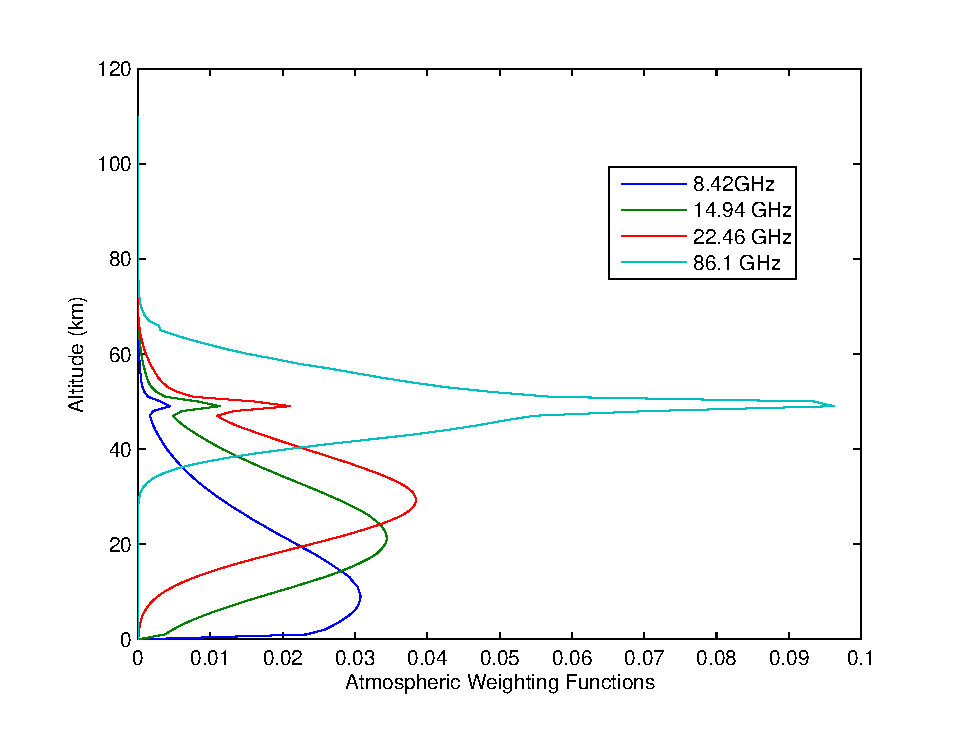
\includegraphics[width=0.7\textwidth]{./rtm/plots/weight.eps}
	\caption{Disk-averaged weighting function of the Venus atmosphere at frequencies of 8.42, 14.94, 22.46, and 86.1 GHz. }
		\label{fig:weight}
\end{figure}

%RTM Theory and shit

%For transfer over a path length $s$ with a surface impact angle $\theta$ the radiative transfer at the top of the atmosphere can then be written as 
%\begin{equation}
%\begin{split}
%I_\nu(s,\theta) =& I_{\nu,surf}\exp(-\tau_\nu(s)) + I_{\nu,sky}\exp(-2\tau_\nu(s))\\
%&+\int_0^s \alpha B_\nu(T) \exp(-tau_\nu(s))ds \\
%&+\int_0^s 
%\end{split}
%\end{equation}